\fancypagestyle{plain}{\fancyhead{}\renewcommand{\headrulewidth}{0pt}}
\chapter{Stato dell'Arte}
In un mondo in cui sempre più dispositivi necessitano di connessione alla rete e i dati personali richiedono un alto livello di protezione, oltre che di elaborazione attraverso l'impiego di algoritmi più o meno complessi, le potenzialità offerte in tale direzione dall'Edge Computing hanno attirato l'attenzione dei colossi del settore.

Google, ad esempio, ha recentemente rilasciato Edge TPU e Cloud IoT Edge \cite{iotgoogle}: il primo è un ASIC creato specificamente per eseguire l'IA a livello periferico, mentre il secondo è una piattaforma per l'Edge Computing che estende le capacità di elaborazione dei dati e Machine Learning (ML) di Google Cloud ai dispositivi perimetrali. L'idea di fondo è quella di costruire i propri modelli sul Cloud, per poi utilizzarli su dispositivi Cloud IoT Edge sfruttando le potenzialità offerte dall'acceleratore hardware Edge TPU. Tale circuito è inoltre in grado di eseguire TensorFlow Lite \cite{tflowlite}: una piattaforma che fornisce un set di strumenti i quali permettono all'utente di convertire modelli di reti neurali TensorFlow in versioni semplificate e ridotte, adatte ai dispositivi Edge \cite{tflowres}.

Amazon, all'interno della sua offerta di servizi Cloud (AWS), mette a disposizione la soluzione IoT Greengrass \cite{aws}, che semplifica l'inferenza di ML in locale sui dispositivi, mediante modelli creati, formati e ottimizzati nel Cloud. L'utente può inoltre utilizzare modelli il cui training viene fatto in prima persona. L'AWS IoT Greengrass dispone del runtime Lambda \cite{lambda}: un gestore di messaggi, accesso alle risorse, ecc. I requisiti minimi a livello hardware sono 1 GHz di frequenza del processore e 128 MB di RAM.

Microsoft mette a disposizione Azure IoT Edge \cite{azure}: un servizio che permette di distribuire i carichi di lavoro del Cloud per eseguirli su dispositivi perimentrali dell'IoT. Il codice di IoT Edge supporta numerosi linguaggi tra cui C, C\#, Java, Node.js e Python, inoltre la latenza è ridotta siccome i dati vengono elaborati in locale, con la possibilità di usare l'architettura hardware Microsoft, Project Brainwave \cite{bwave}. I dispositivi perimetrali possono poi anche funzionare in condizioni di connessione a internet scarsa, grazie alla gestione dei dispositivi di Azure che sincronizza in automatico lo stato più recente degli apparecchi dopo la riconnessione a internet. Microsoft ha inoltre rilasciato EdgeML \cite{edgeml}: una suite di algoritmi di ML progettata per un utilizzo in situazioni di risorse ridotte. I risultati pubblicati sull'uso di EdgeML per il training su Cloud in condizioni di limitata potenza di calcolo \cite{edgemlres}. Al momento tale libreria prevede algoritmi di tipo k-Nearest Neighbors (kNN) per classificazione, regressione e ranking noti con i nomi di Bonsai, ProtoNN e Robust PCA \cite{edgemlalg}.

In ultimo, IBM ha sviluppato IBM Edge Application Manager \cite{IBM}: una piattaforma intelligente, sicura e flessibile che fornisce uno strumento di gestione per l'elaborazione perimetrale. La soluzione proposta è autonoma, ossia consente ad un singolo amministratore di gestire scalabilità, variabilità e frequenza di modifica degli ambienti delle applicazioni su decine di migliaia di endpoint. Gli endpoint perimetrali si eseguono su contenitori Red Hat OpenShift \cite{redhat}. IBM Edge Application Manager supporta inoltre tool di IA per Deep Learning e riconoscimento di voce e immagini, oltre all'analisi video e acustica.

Anche nella letteratura scientifica è possibile reperire numerosi articoli pubblicati nel periodo recente, a indicare un orientamento in direzione Edge Computing.

In particolare, riguardo la possibilità di eseguire codice multipiattaforma che sfrutti le potenzialità offerte da questo approccio, si fa riferimento ad un articolo riguardante lo sviluppo di algoritmi di allocazione risorse per migliorare le prestazioni delle Vehicular Networks \cite{VN}. Per la selezione della piattaforma di esecuzione (es. Cloud Computing, Mobile Edge Computing, o Local Computing) viene utilizzato l'algoritmo k-Nearest Neighbor (kNN), mentre, per il problema di allocazione delle risorse computazionali, il Reinforcement Learning (RL). I risultati della simulazione mostrano che, rispetto all'algoritmo di base in cui tutte le attività vengono eseguite sul server di Edge Computing locale o mobile, lo schema di allocazione delle risorse consente una riduzione significativa della latenza che si attesta intorno all'80\%.

Per far fronte al problema del consumo di energia dei device IoT, l'approccio Edge Computing è stato trattato al'interno di un articolo di Olli Väänänen e Timo Hämäläinen \cite{energyIoT}. Aspetto importante di tale ricerca è la focalizzazione sul concetto di virtualizzazione. L'approccio consigliato è quello della container-based virtualization: ambienti di sviluppo virtuali emulano un determinato sistema operativo (OS), in questo modo è possibile produrre codice indipendente dalla piattaforma. I container possono essere eseguiti da dispositivi dotati di risorse limitate (es. Raspberry Pi), tuttavia richiedono una certa potenza computazionale e un generico OS.

Un ulteriore aspetto critico riguardante l'Edge Computing è il coordinamento tra dispositivi. Nell'ambito dei vari modelli che è possibile adottare, quelli tuple-based sono i più conosciuti e utilizzati, principalmente per la loro flessibilità \cite{tuple}. Ne è un esempio il modello Tusow (Tuple Spaces over the Web) \cite{tusow}. Le tuple rappresentano i messaggi o i dati scambiati tra i componenti e l'interazione tra gli stessi è gestita definendo come e quando i vari agenti coinvolti sono in grado di inserire, leggere o elaborare i dati. Tusow permette ai vari clients di rappresentare le tuple in diversi formati: YAML, JSON, XML, FOL e plain text. Il supporto multipiattaforma offerto da tale sistema mira a fornire un mezzo di interazione ad alto livello per clients eterogenei, permettendo agli sviluppatori di non curarsi delle complessità intrinseche della rete di basso livello.

La ricerca scientifica si sta orientando verso l'implementazione di algoritmi di ML applicati all'Edge Computing, come anche dimostrato dalle proposte di Google e Microsoft in tale ambito \cite{tflowres}, \cite{edgemlres}.
È stata ad esempio testata la possibilità di eseguire algoritmi di ML su Raspberry Pi \cite{mlrasp}. In particolare sono stati implementati tre algoritmi: Support Vector Machine (SVM), Multi-Layer Perceptron e Random Forest, raggiungendo una precisione oltre l'80\% mantenendo però un basso consumo di energia.

È stato inoltre analizzato un approccio di Deep Learning in cui vengono utilizzati autoencoder a livello Edge in modo da operare una riduzione delle dimensioni dei dati \cite{encoder}, portando benefici in termini di tempo e spazio richiesti. Tale progetto illustra tre differenti scenari. Nel primo, dati provenienti da sensori vengono mandati a dei "nodi Edge", dove viene applicata la riduzione delle dimensioni, per poi applicare le tecniche di ML su Cloud. Nel secondo, i dati che sono stati ridotti in Edge vengono trattati sul Cloud in modo da riottenere i dati originari per poi successivamente applicare il ML. Nel terzo ed ultimo caso invece, la tecnica utilizzata è quella del Cloud Computing: i dati vengono mandati dai sensori direttamente al Cloud. I risultati finali mostrano come l'utilizzo di autoencoder a livello Edge riduca il numero di features e, di conseguenza, l'ammontare di dati inviati al Cloud.

In ultimo, Respiro è un inalatore smart prodotto da Amiko \cite{respiro} che contiene un processore ultra-low-power ARM Cortex-M. Tale inalatore fa affidamento sul ML per interpretare le vibrazioni provenienti dal sensore posto al suo interno. Il dispositivo è addestrato per riconoscere diverse tipologie di respiro e calcolare di conseguenza importanti parametri in ambito medico come la capacità polmonare e la tecnica di inalazione. I dati così prodotti vengono poi processati da un'applicazione e, se la connessione lo permette, inviati al Cloud per essere conservati ed elaborati potendoli confrontare inoltre con i risultati altrui a fini statistici. Infine, attraverso l'app, viene inviato un feedback all'utente affinché possa avere sotto controllo i dati estrapolati.

Queste sono le principali soluzioni disponibili nel mercato tecnologico e nelle più recenti ricerche accademiche. È possibile notare come gli aspetti ritenuti più importanti siano l'ottimizzazione delle risorse, il basso consumo di energia, l'indipendenza dalla piattaforma, la privacy e la bassa latenza, oltre alla facilità di utilizzo.

Edge Engine nasce con l'idea di creare un runtime system slegato dalla piattaforma che soddisfi i requisiti cardine dell'Edge Computing sopracitati. A differenza delle soluzioni appena presentate, questo progetto cerca di fornire un software completamente personalizzabile e adattabile a qualsiasi apparato IoT, come riassunto dallo schema visibile in figura \ref{edgecomplete}.

\begin{figure}
	\centering
	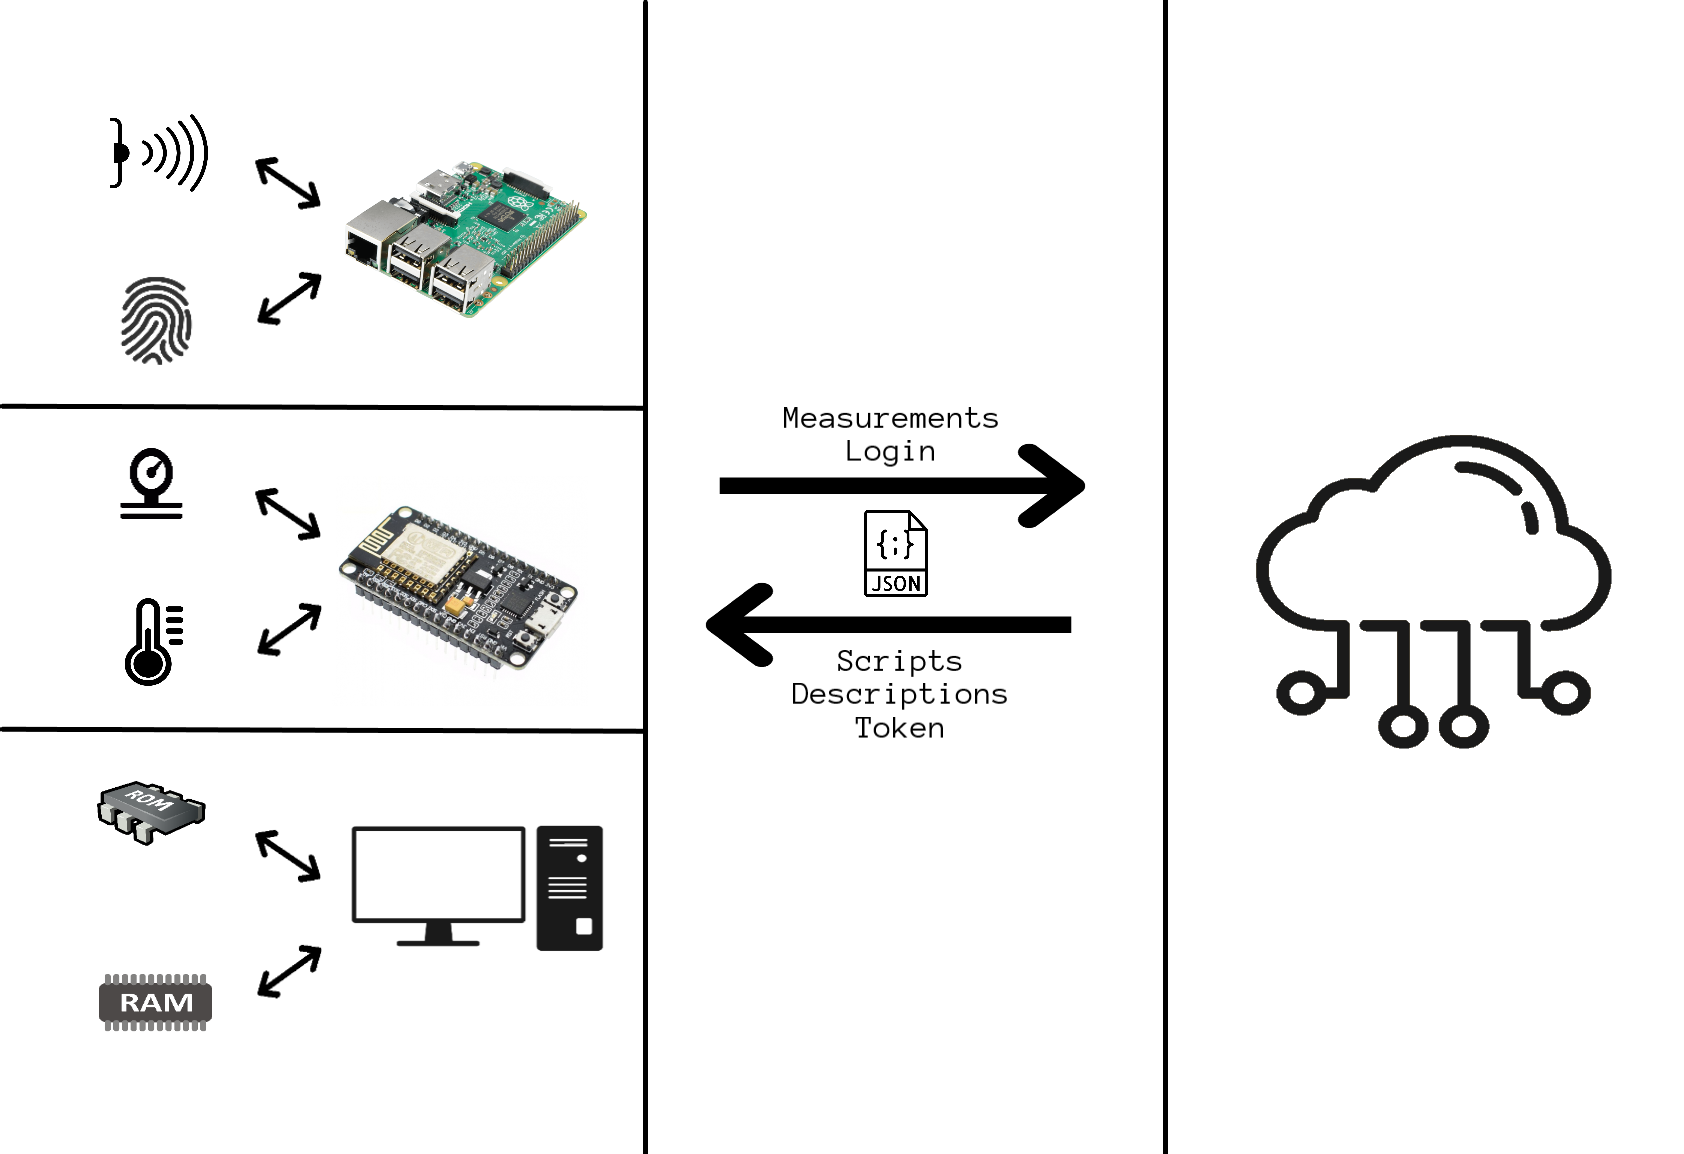
\includegraphics[width=\linewidth]{pics/edgineCP}
	\caption{Schema funzionale di Edge Engine su piattaforme eterogenee}
	\label{edgecomplete}
\end{figure}